% !TeX spellcheck = ru_RU
% !TEX root = vkr.tex

\section{Эксперимент}

Целями следующих экспериментов является выявление возможности зависимости пропускной способности рантайма от взаимодействия воркеров с глобальной очередью. Это взаимодействие будет оцениваться c помощью выделенных метрик.

Каждая задача спавнер помещается в отдельный блокирующий поток путем вызова \verb|spawn_blocking| и спецификации рантайму \verb|max_blocking_threads| равному количеству спавнеров. Каждая задача продуцирует одинаковое количество пустых листовых задач. Дабы избежать оптимизации редуцирующей тело задачи в нее помещена непрозрачная для компилятора функция-пустышка \verb|std::hint:black_box|.

\subsection{Условия эксперимента}

Исследования проводились на системе TODO, процессор: TODO. Проект был собран с флагом \verb|--release|.Бенчмарк был запущен с значением \verb|nice| равным минус двадцати.

Машина для измерение производительности была любезно предоставлена командой \verb|TATLIN.BACKUP| и находилась удаленно, в связи с чем на ней было невозможно отключение сети.

\subsubsection{Метрики семплирования}

Каждую итерацию семплирования предваряли тридцать итераций прогрева. Семплирование представило собой запуск дополнительного системного потока, опрашивающего рантайм каждые пятьсот наносекунд на протяжении исполнения им задач. Всего было выполнено сто итераций.

\subsubsection{Тотальные метрики}

Тотальные метрики были получены путем произведения тридцати итераций прогрева с последующими ста итерациями исполнения на отдельном инстансе рантайма, после чего метрики подвергались экстракции из последнего.

\subsection{Ход исследования}

\begin{figure}[H]
    \begin{center}
        \makebox[\textwidth]{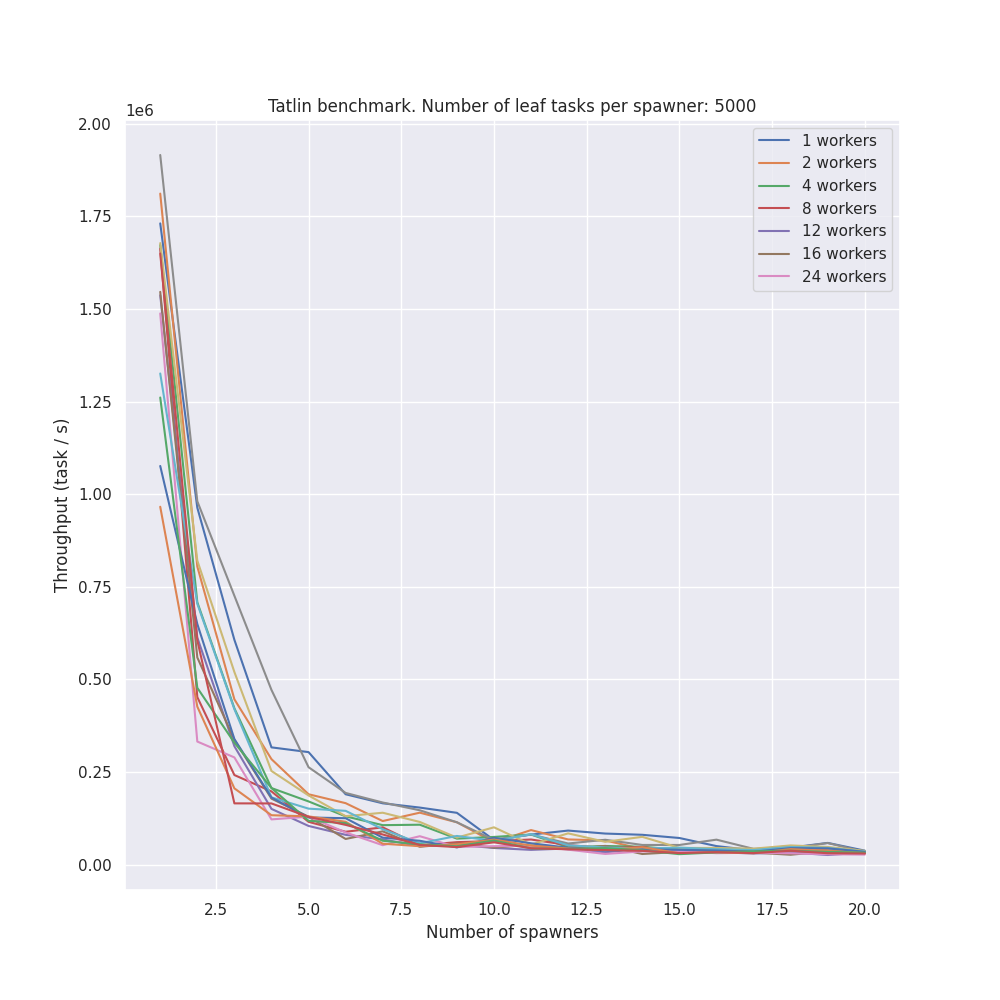
\includegraphics[scale=0.55]{pictures/blocking/tatlin_blocking.png}}
    \end{center}

    \caption{Пропускная способность в зависимости от количества воркеров и спавнеров}
    \label{fig:tatlin:line:nspawn:5000}
\end{figure}

Как видно из графика \ref{fig:tatlin:line:nspawn:5000} пропускная способность рантайма падает с увеличением спавнеров независимо от количества воркеров. Источником задач в данном случае является глобальная очередь. Воркеры могу делиться задачами с помощью механизма стилинга, однако получать новые задачи они способны исключительно благодаря взаимодействию с глобальной очередью.
